\documentclass{article}
\title{Tendencias Global Management And Entreprenurship \\ \Huge{``Flexitarianism''}}
\author{David Gabriel Corzo Mcmath}
\date{2020-Jan-20 22:49:48}
%%%%%%%%%%%%%%%%%%%%%%%%%%%%%%%%%%%%%%%%%%%%%%%%%%%%%%%%%%%%%%%%%%%%%%%%%%%%%%%%%%%%%%%%%%%%%%%%%%%%%%%%%%%%%%%%%%%%%%%%%%%%%%%%%%%%%%%%%%%%%%%
\usepackage[margin = 1in]{geometry}
\usepackage{graphicx}
\usepackage{fontenc}
\usepackage{pdfpages}
\usepackage[spanish]{babel}
\usepackage{amsmath}
\usepackage{amsthm}
\usepackage[utf8]{inputenc}
\usepackage{enumitem}
\usepackage{mathtools}
\usepackage{import}
\usepackage{xifthen}
\usepackage{pdfpages}
\usepackage{transparent}
\usepackage{color}
\usepackage{fancyhdr}
\usepackage{lipsum}
\usepackage{sectsty}
\usepackage{titlesec}
\usepackage{calc}
\usepackage{lmodern}
\usepackage{xpatch}
\usepackage{blindtext}
\usepackage{bookmark}
\usepackage{fancyhdr}
\usepackage{xcolor}
\usepackage{tikz}
\usepackage{blindtext}
\usepackage{hyperref}
\usepackage{listing}
\usepackage{spverbatim}
\usepackage{fancyvrb}
\usepackage{fvextra}
\usepackage{amssymb}
\usepackage{pifont}
\usepackage{longtable}
\usepackage{etoolbox}
\gappto{\UrlBreaks}{\UrlOrds}
%%%%%%%%%%%%%%%%%%%%%%%%%%%%%%%%%%%%%%%%%%%%%%%%%%%%%%%%%%%%%%%%%%%%%%%%%%%%%%%%%%%%%%%%%%%%%%%%%%%%%%%%%%%%%%%%%%%%%%%%%%%%%%%%%%%%%%%%%%%%%%%
\begin{document}
\maketitle

\section{Explicación de tendencias el medio ambiente}
Recientemente, se ha estado dando una gran ola de gente que quiere comprar productos que sean ``ambientalmente limpios'' por que la consciencia del medio ambiente ha estado en constante aumento. Según National Geographic se fundamenta esta afirmación con estadísticas que muestran que ha ocurrido un aumento de hasta 9\% en la consciencia del medio ambiente principalmente por el asunto del calentamiento global.

%%%%%%%%%%%%%%%%%%%%%%%%%%%%%%%%%%%%%%%%%%%%%%%%%%%%%%%%%%%%%%%%%%%%%%%%%%%%%%%%%%%%%%%%%%%%%%%%
\section{Autoconciencia del medio ambiente - Tendencias }
\emph{Citación:``The percentage of Americans who say global warming is personally important is now at a record high, 72 percent, up 9 percentage points since March 2018'' - Anthony Leiserowitz Director de Climate Change Communication en Yale} Fuente: Anexos [1] . Dado a este hecho revelador se puede entonces manifestar objetivamente la demanda y la tendencias a que las personas tengan una orientación a querer hacer todo lo que puedan para mejorar el medio ambiente, productos como pajíllas metálicas que son lavables han estado en aumento también, cosas como legislación en contra de la venta de pajíllas de plástico han estado en constante aumento alrededor del mundo, localmente en Guatemala se han impuesto fuertes regulaciones en contra del uso de pajíllas de plástico, restaurantes están dando pajíllas hechas de materia biodegradable por lo mismo. Fuente: Anexos [2]. En particular esto es relevante por que una razón muy popular que las personas usan para justificar el \emph{flexivegetarianismo} la ayuda que brinda al no liberar gases como metano producido por ciertos productos animales, por esto la persona \emph{ambientalmente consciente} le tiende a atraer la opción del \emph{flexivegetarianismo}. 

%%%%%%%%%%%%%%%%%%%%%%%%%%%%%%%%%%%%%%%%%%%%%%%%%%%%%%%%%%%%%%%%%%%%%%%%%%%%%%%%%%%%%%%%%%%%%%%%

\subsection{Identificar tendencias $\rightarrow$  Al vegetarianismo flexible}
Entonces en esta nueva tendencia que se identifica se producen nuevas corrientes de costumbre y una que ha estado en constante aumento ha sido el ``Flexitarianism'' que sostiene la idea de comer de una manera \emph{pseudo-vegetariana} por motivos como ayudar al medio ambiente y salud, dichos \emph{flexivegetarianos} intentan mantener dietas vegetarianas pero ocasionalmente deleitarse con algún producto animal. Es por ende que se deduce que el ``Flex'' en la palabra muy probablemente sea por que son más flexibles que los vegetarianos. De acuerdo con las estadísticas la cantidad de personas interesadas en ser vegetarianas están en aumento desde el 2017, pero entre los vastos sacrificios que hay que hacer para volverse puramente vegetariano esta la renuncia a comer productos animales, por esto se vuelve muy difícil poder hacer la transición a esta nueva forma de vivir, pero talvés las personas puedan emplear una alternativa más moderada a esta decisión y esta podría ser el \emph{flexitarianismo}; Fuente: Anexos [3].  Apreciar en la figura \ref{veg} presentada a continuación se observa el número de personas interesadas en volverse vegetarianas a lo largo del tiempo, se aprecia que está efectivamente en aumento respecto a las otras dietas de esta misma índole.  
\begin{figure}[htbp]
    \centering
    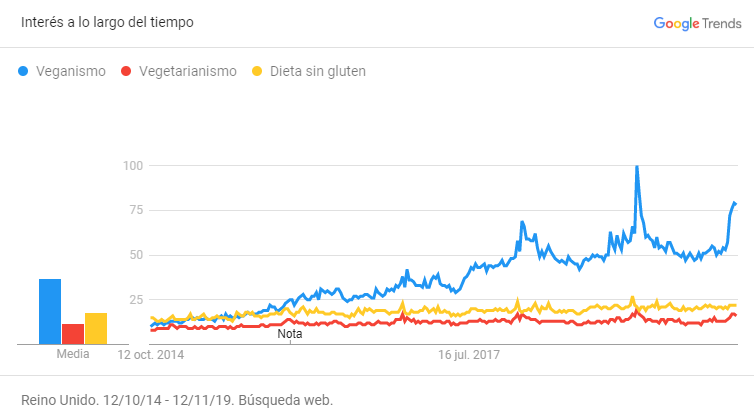
\includegraphics[width=12cm]{./TendenciasVegetarianas.png}
    \caption{Tendencias de interés al vegetarianismo}
    \label{veg}
\end{figure}

%%%%%%%%%%%%%%%%%%%%%%%%%%%%%%%%%%%%%%%%%%%%%%%%%%%%%%%%%%%%%%%%%%%%%%%%%%%%%%%%%%%%%%%%%%%%%%%%
\subsection{Productos vegetarianos en el mercado}
Según recientes estadísticas conducidas en diciembre de 2019 se pudo medir aproximadamente cuánta demanda se calcula tener actualmente de productos vegetarianos, en 2014 la estadística concluyó que habían un 1\% de vegetarianos en EEUU por lo que ahora sea una 6\% significa que el número tuvo un aumento de 500\% entre esos cinco años. No solo se presentan aumentos en EEUU sino también en países como Inglaterra. Fuente: Anexos [4].

%%%%%%%%%%%%%%%%%%%%%%%%%%%%%%%%%%%%%%%%%%%%%%%%%%%%%%%%%%%%%%%%%%%%%%%%%%%%%%%%%%%%%%%%%%%%%%%%
\section{Oportunidad de negocio}
Según la información presente se proponen ideas en el ámplio mundo económico, estas ideas pueden ser buenas y pueden ser malas pero sólo un juez existe en este caso y se llama el proceso de mercado, por ende las oportunidades de mercado que se pueden aprovechar en mi opinión son las siguientes.

\subsection{Oportunidad y propuesta de negocio \#1}
Dado al vasto mercado que ha surgido por el aumento de popularidad del vegetarianismo, el \emph{flexivegetarianismo} resulta ser más fácil de vender por conllevar menos costos de transacción al querer cambiar de estilo de vida a la de \emph{flexivegetarianismo}. Entonces lo que propongo es el lanzamiento de una aplicación digital móvil y web con ciertas funcionalidades claves que mantengan motivado al usuario de mantenerse en esta dieta por medio de medición de progreso, medición de ``qué tanto está ayudando al medio ambiente'', ayuda nutricional y asistencia.

\subsection{Oportunidad y propuesta de negocio \#2}
Según la información presentada anteriormente se podría especular que tendría buena demanda hacer algún tipo de retiro para que una persona interesada pueda tomar un descanso y ser introducida con menos resistencia al nuevo estilo de vida del \emph{flexivegetarianismo}. Propongo tener un campo en el que las personas puedan pagar un retiro para ser introducidos al nuevo estilo de vida mientras están descansando.

\subsection{Oportunidad y propuesta de negocios \#3}
Dado a la nueva demanda de productos vegetarianos o \emph{flexivegetarianos} se podría introducir al mercado un supermercado hecho para esta nueva corriente de costumbre \emph{flexivegetariana}. Propongo trabajar con empresas de supermercado locales para introducir estos nuevos productos al mercado.


%%%%%%%%%%%%%%%%%%%%%%%%%%%%%%%%%%%%%%%%%%%%%%%%%%%%%%%%%%%%%%%%%%%%%%%%%%%%%%%%%%%%%%%%%%%%%%%%
\section{Anexos}
\begin{enumerate}[label={[\arabic*]}]
    \item \url{https://www.nationalgeographic.com/environment/2019/01/climate-change-awareness-polls-show-rising-concern-for-global-warming/}
    \item \url{https://www.nationalgeographic.com/environment/2018/07/news-plastic-drinking-straw-history-ban/} 
    \item \url{https://www.vegansociety.com/news/media/statistics}  
    \item \url{https://plantproteins.co/vegan-plant-based-diet-statistics/}
\end{enumerate}




















\end{document}
